\documentclass[conference,a4paper]{IEEEtran}

% Escritura mejorada de fórmulas matemáticas
\usepackage{amsmath}

% Inserción de gráficos
\usepackage{graphicx}

% Escritura de pseudocódigo
\usepackage[kw]{pseudo}

% Escritura mejorada de tablas
\usepackage{booktabs}

% Escritura mejorada de citas bibliográficas
\usepackage{cite}


% Macros traducidas
\def\contentsname{Índice general}
\def\listfigurename{Índice de figuras}
\def\listtablename{Índice de tablas}
\def\refname{Referencias}
\def\indexname{Índice alfabético}
\def\figurename{Fig.}
\def\tablename{TABLA}
\def\partname{Parte}
\def\appendixname{Apéndice}
\def\abstractname{Resumen}
% IEEE specific names
\def\IEEEkeywordsname{Palabras clave}
\def\IEEEproofname{Demostración}


\begin{document}


\title{Clasificación Relacional de Documentos Científicos: Un Enfoque Topológico sobre el Dataset Cora}


\author{
  \IEEEauthorblockN{Juan Antonio Fernández Ruiz}
  \IEEEauthorblockA{
    \textit{Dpto. Ciencias de la Computación e Inteligencia Artificial}\\
    \textit{Universidad de Sevilla}\\
    Sevilla, España\\
    juanafr@us.es}
  
  \and
  
  \IEEEauthorblockN{Nombre y apellidos alumno 2}
  \IEEEauthorblockA{
    \textit{Dpto. Ciencias de la Computación e Inteligencia Artificial}\\
    \textit{Universidad de Sevilla}\\
    Sevilla, España\\
    Correos electrónicos UVUS y de contacto (si distinto)}
}

\maketitle
\thispagestyle{plain} % fuerza número en la primera página
\pagestyle{plain}     % resto de páginas


% Resumen
\begin{abstract}
  Este documento presenta los avances preliminares en la construcción y evaluación de modelos
  de aprendizaje automático relacional aplicados al conjunto de datos Cora. El objetivo 
  principal es predecir la temática de artículos científicos combinando sus atributos 
  textuales con características topológicas extraídas de su red de citas. Hasta la fase 
  actual de desarrollo, se ha completado el análisis exploratorio, la extracción de métricas 
  estructurales (centralidad, clustering y comunidades) y el establecimiento de una línea 
  base de rendimiento mediante cuatro algoritmos clásicos de clasificación. Los resultados 
  preliminares muestran que los Árboles de Decisión logran generalizar de manera competitiva 
  frente a modelos conexionistas y probabilísticos.
\end{abstract}


% Palabras claves
\begin{IEEEkeywords}
  Aprendizaje Automático Relacional, Teoría de Grafos, Clasificación de Nodos, Dataset Cora.
\end{IEEEkeywords}


\section{Introducción}

El análisis de datos estructurados en forma de red se ha convertido en un área de vital importancia 
debido a la ubicuidad de los grafos en dominios como las redes sociales, biológicas y de comunicaciones.
A diferencia del aprendizaje automático tradicional, que asume la independencia entre los ejemplos, 
el aprendizaje relacional aprovecha las correlaciones inherentes en los enlaces entre nodos para mejorar
la capacidad predictiva de los modelos.

En numerosos grafos del mundo real aparece el fenómeno conocido como *homofilia*, según el cual los nodos conectados tienden a compartir características similares. En redes de citas científicas como el dataset Cora, este comportamiento se manifiesta en que los artículos pertenecientes a una misma temática suelen citar trabajos relacionados del mismo ámbito de investigación.

Esta propiedad resulta especialmente relevante en nuestro contexto, ya que permite aprovechar no solo las características individuales de cada nodo, sino también la información estructural derivada de sus conexiones. Las *Graph Neural Networks* (GNNs) explotan precisamente esta dependencia relacional mediante mecanismos de agregación de vecindario, propagando información entre nodos próximos del grafo para mejorar tareas como la clasificación de documentos.

En este trabajo, se aborda el problema de la clasificación de nodos en redes de citación científica
utilizando el conjunto de datos Cora. El enfoque adoptado consiste en la extracción manual de características
topológicas para enriquecer las propiedades nativas de los documentos. El resto de este documento detalla los
preliminares teóricos (Sección II), la metodología y decisiones de diseño adoptadas hasta la fecha (Sección III), 
los resultados empíricos preliminares (Sección IV) y, finalmente, las conclusiones e hitos de trabajo futuro (Sección V).

\section{Preliminares}
\subsection{Métodos empleados}
Para la representación y procesamiento de los datos relacionales se ha empleado la librería de Python \textit{NetworkX}. 
Específicamente, nos apoyamos en la teoría de grafos para calcular medidas topológicas de centralidad, densidad local
(coeficiente de \textit{clustering}) y algoritmos de detección de comunidades para identificar subestructuras cohesivas.
Para la etapa de modelado y clasificación, se ha empleado \textit{Scikit-Learn}, evaluando algoritmos basados en instancias
(\textit{k-Vecinos más Cercanos}), particionado recursivo (\textit{Árboles de Decisión}), aproximaciones probabilísticas 
(\textit{Naive Bayes} Gaussiano) y modelos conexionistas (\textit{Perceptrón Multicapa}).
\subsection{Trabajo Relacionado}

Como referencia fundamental para nuestro enfoque, destaca el trabajo de Sen \textit{et al.} sobre clasificación colectiva en datos
de redes, en el cual los autores emplean el conjunto de datos Cora para predecir la temática de los artículos basándose en 
la correlación de sus enlaces y propiedades. Su investigación demuestra que aprovechar la estructura subyacente de la red 
mejora significativamente el rendimiento frente a clasificadores tradicionales que tratan cada documento de forma independiente.

La clasificación de nodos en grafos constituye uno de los problemas más relevantes dentro del aprendizaje automático sobre estructuras 
relacionales. A diferencia de los enfoques tradicionales de aprendizaje supervisado, donde cada instancia se considera de manera 
independiente, en los grafos existe información adicional derivada de las relaciones entre nodos, lo que permite explotar dependencias 
estructurales durante el proceso de aprendizaje.

En muchos grafos reales aparece el fenómeno conocido como \textit{homofilia}, según el cual los nodos conectados tienden a compartir 
propiedades similares. En redes de citas científicas como el dataset Cora, esta propiedad se manifiesta en que artículos pertenecientes 
a áreas temáticas similares suelen citar trabajos relacionados del mismo ámbito de investigación. Como consecuencia, la estructura del 
grafo aporta información semántica complementaria a las características propias de cada nodo.

La clasificación de nodos puede abordarse explotando diferentes tipos de correlaciones presentes en la red. De forma general, 
pueden distinguirse tres fuentes principales de información: (1) los atributos propios del nodo, (2) los atributos de los nodos vecinos 
y (3) las etiquetas de los nodos vecinos. Mientras que los enfoques clásicos de aprendizaje automático se centran únicamente en las
características individuales de cada instancia, los modelos basados en grafos incorporan además información contextual derivada de la 
conectividad entre nodos.

Las \textit{Graph Neural Networks} (GNNs) explotan precisamente estas dependencias relacionales mediante mecanismos de agregación y
propagación de información entre vecinos, conocidos como \textit{message passing}. En este proceso, cada nodo actualiza iterativamente 
su representación interna utilizando tanto sus propias características como la información agregada de su vecindario local.

Entre las arquitecturas más relevantes destacan las \textit{Graph Convolutional Networks} (GCN), que introducen operaciones 
convolucionales adaptadas a grafos mediante normalización de la matriz de adyacencia, y modelos posteriores como GraphSAGE, 
que permiten generalizar el aprendizaje mediante funciones de agregación inductivas.

En este trabajo se estudia el aprovechamiento de las dos primeras fuentes de correlación: los atributos propios 
de cada nodo y los atributos de sus vecinos dentro de la estructura del grafo. Para ello se emplea el dataset Cora, ampliamente utilizado 
como benchmark en tareas de clasificación de nodos sobre grafos homofílicos.


\section{Metodología}


\section*{A. Dataset Cora y Análisis Exploratorio}

El conjunto de datos Cora original consta de 2708 publicaciones científicas divididas en 7 clases temáticas, vinculadas mediante 5429 
enlaces de citación. La matriz de propiedades nativas de los documentos está compuesta por un vocabulario binario de 1433 palabras.

El análisis exploratorio reveló una extrema dispersión en los datos textuales, con un 98.73\% de ceros y un promedio de solo 18.17 palabras
clave presentes por artículo. Además, se evidenció un marcado desbalanceo de clases, siendo \textit{Neural\_Networks} la clase dominante 
con 818 artículos, frente a temáticas marcadamente minoritarias como \textit{Rule\_Learning} con 180 instancias (Fig.~\ref{fig:dist-clases}).

Asimismo, la distribución del número de palabras activas por documento (Fig.~\ref{fig:dist-palabras}) confirma la alta dispersión del espacio
de atributos nativos, con una fuerte concentración en valores bajos.

\begin{figure}
  \centering
  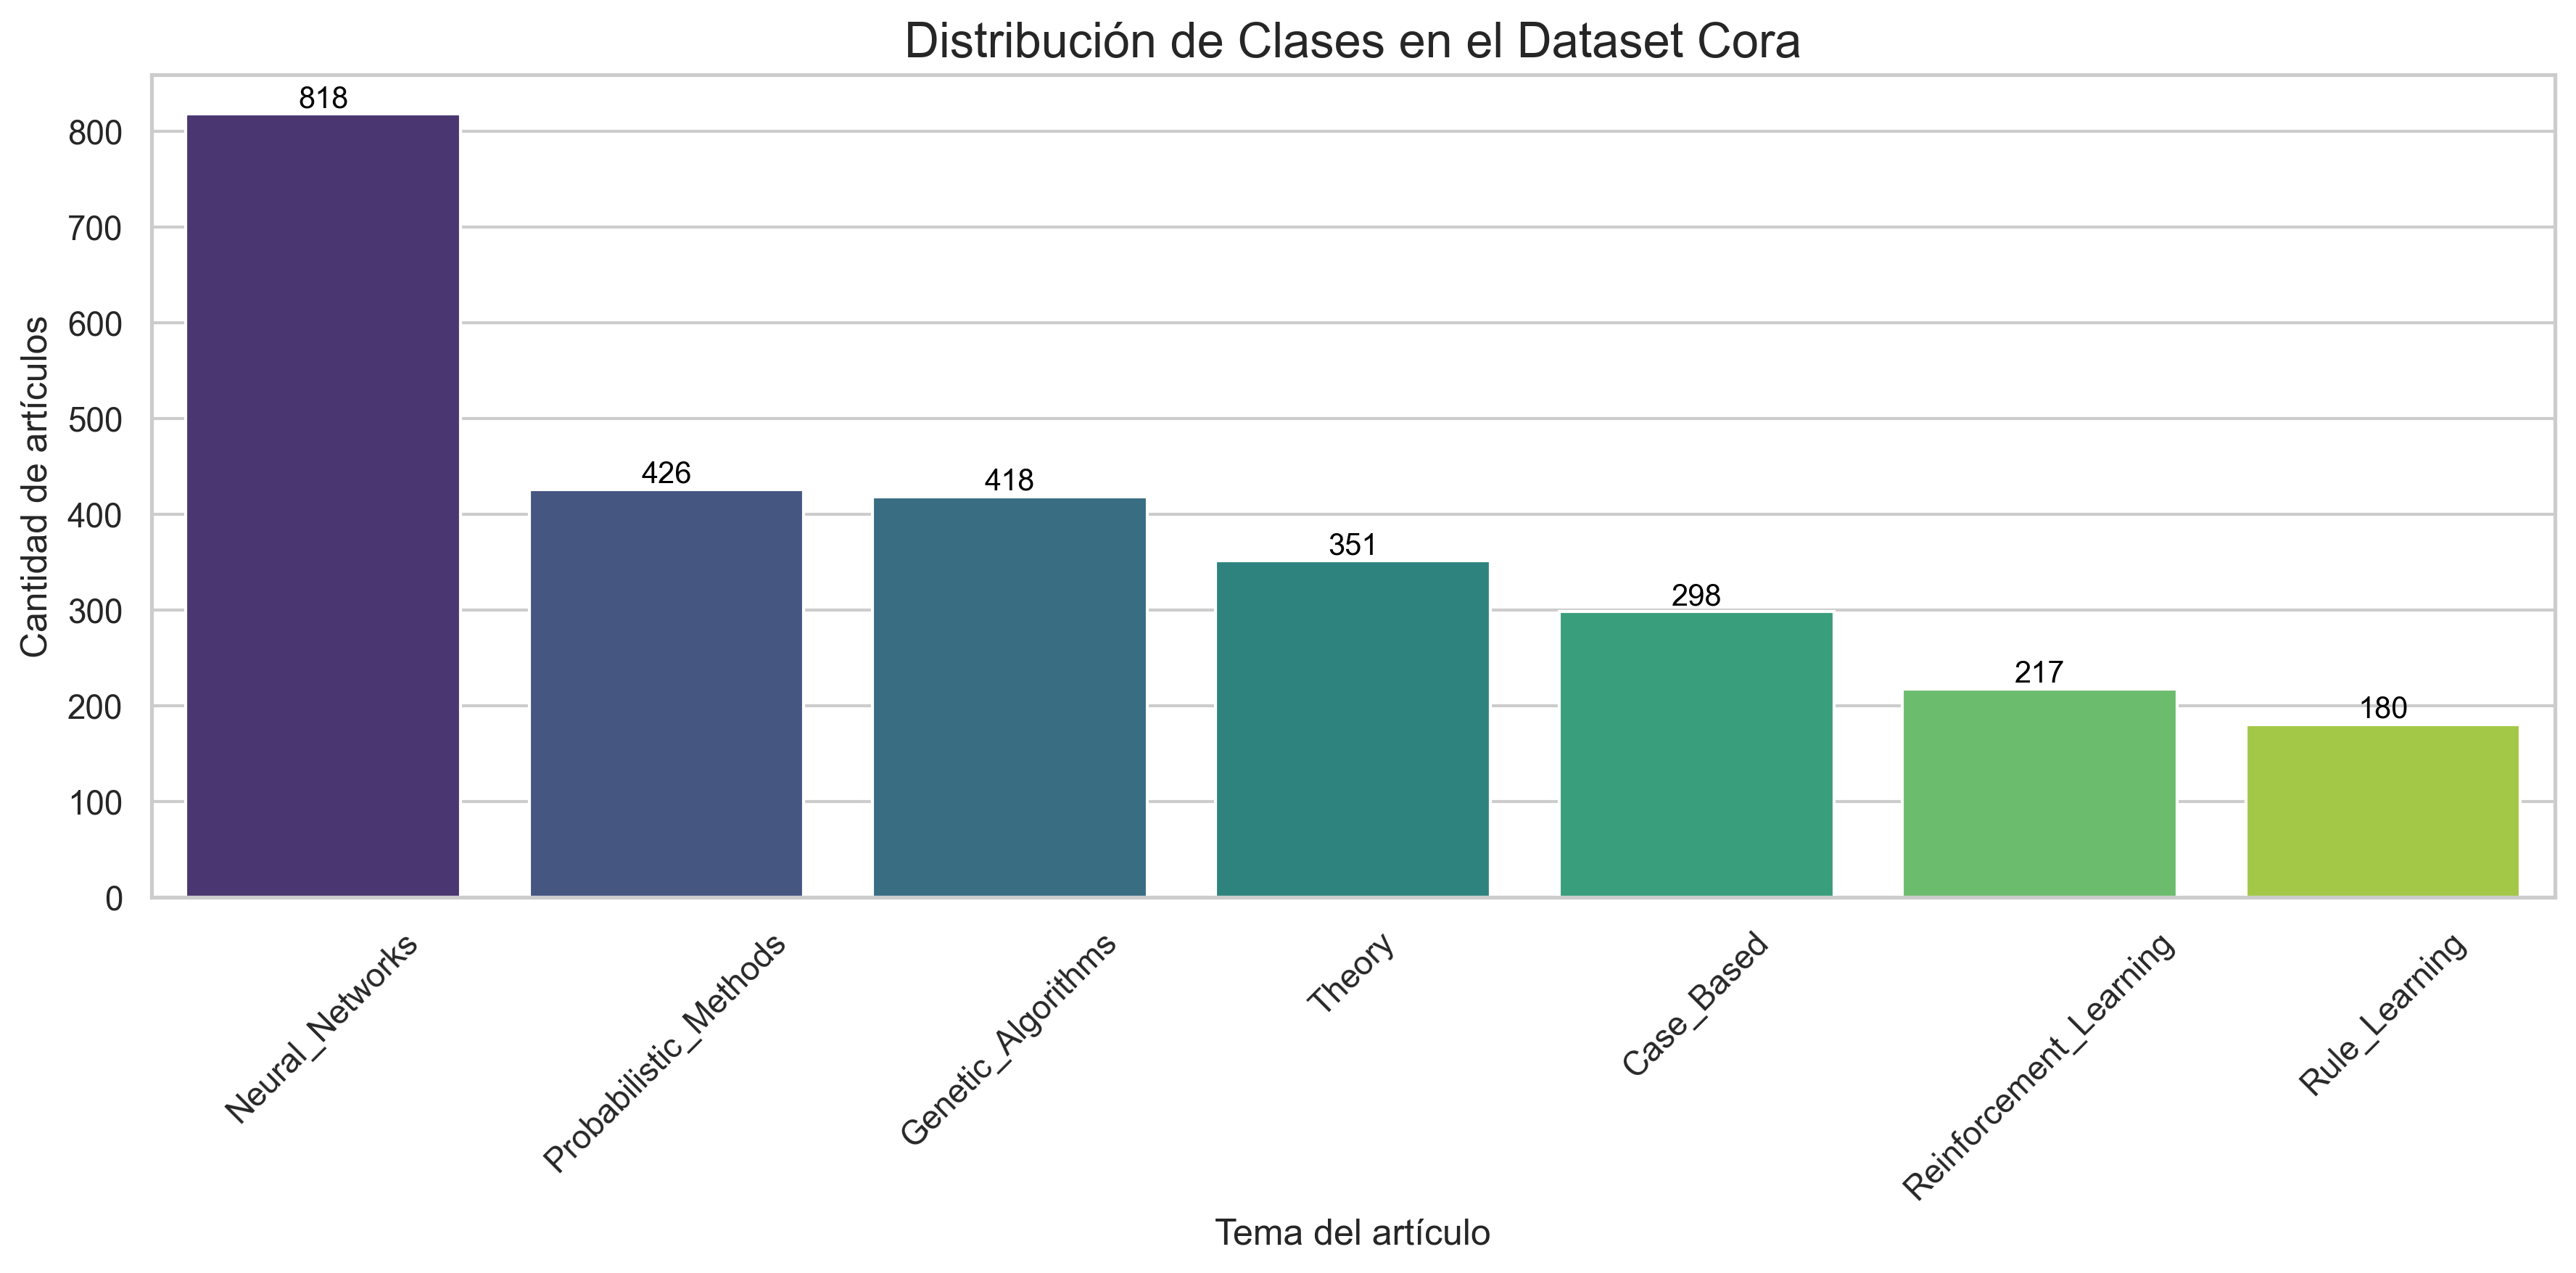
\includegraphics[width=\columnwidth]{figuras/distribucion_clases_cora.png}
  \caption{Distribución de clases del dataset Cora}
  \label{fig:dist-clases}
\end{figure}

\begin{figure}
  \centering
  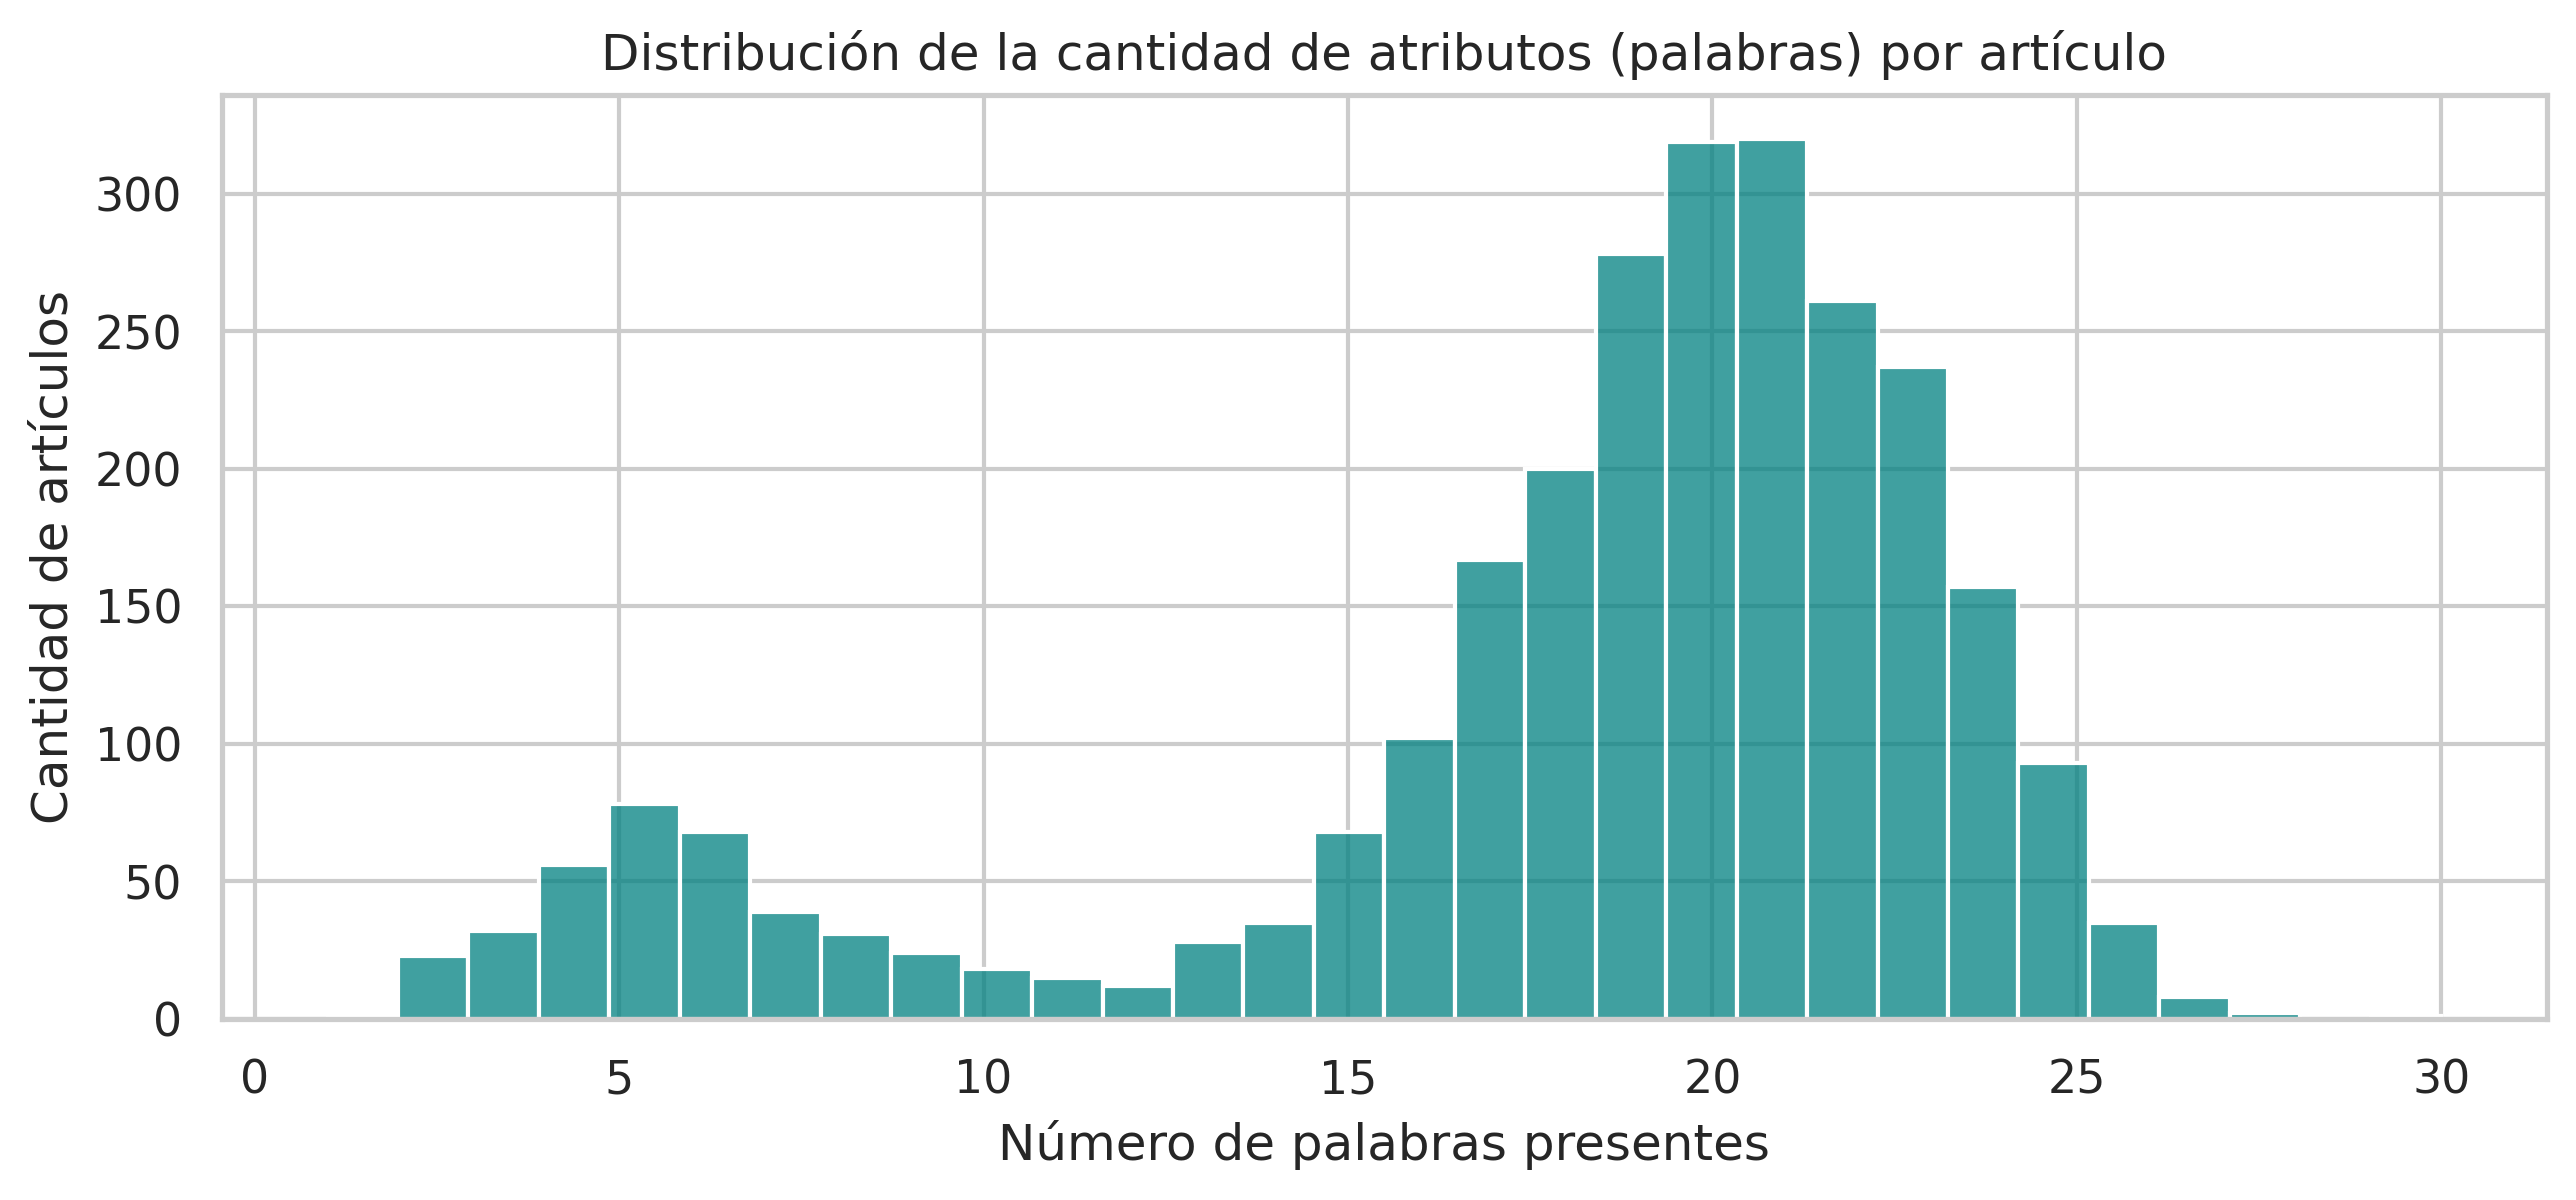
\includegraphics[width=\columnwidth]{figuras/distribucion_palabras_por_articulo_cora.png}
  \caption{Distribución de palabras activas por artículo en Cora}
  \label{fig:dist-palabras}
\end{figure}

\section*{B. Arquitectura Usada y Extracción de Características}

Para la representación matemática de la información, se tomó la decisión de diseño de modelar la red de citas como un grafo no dirigido. 
Esta arquitectura de los datos permitió la fusión de forma natural de las citas recíprocas en 5278 aristas únicas y garantizó la 
convergencia estructural para los algoritmos topológicos aplicados posteriormente. La distribución de grados observada en la red
(Fig.~\ref{fig:dist-grados}) evidencia una topología heterogénea, coherente con la utilidad de métricas de centralidad para caracterizar
la influencia estructural de cada nodo.

\begin{figure}
  \centering
  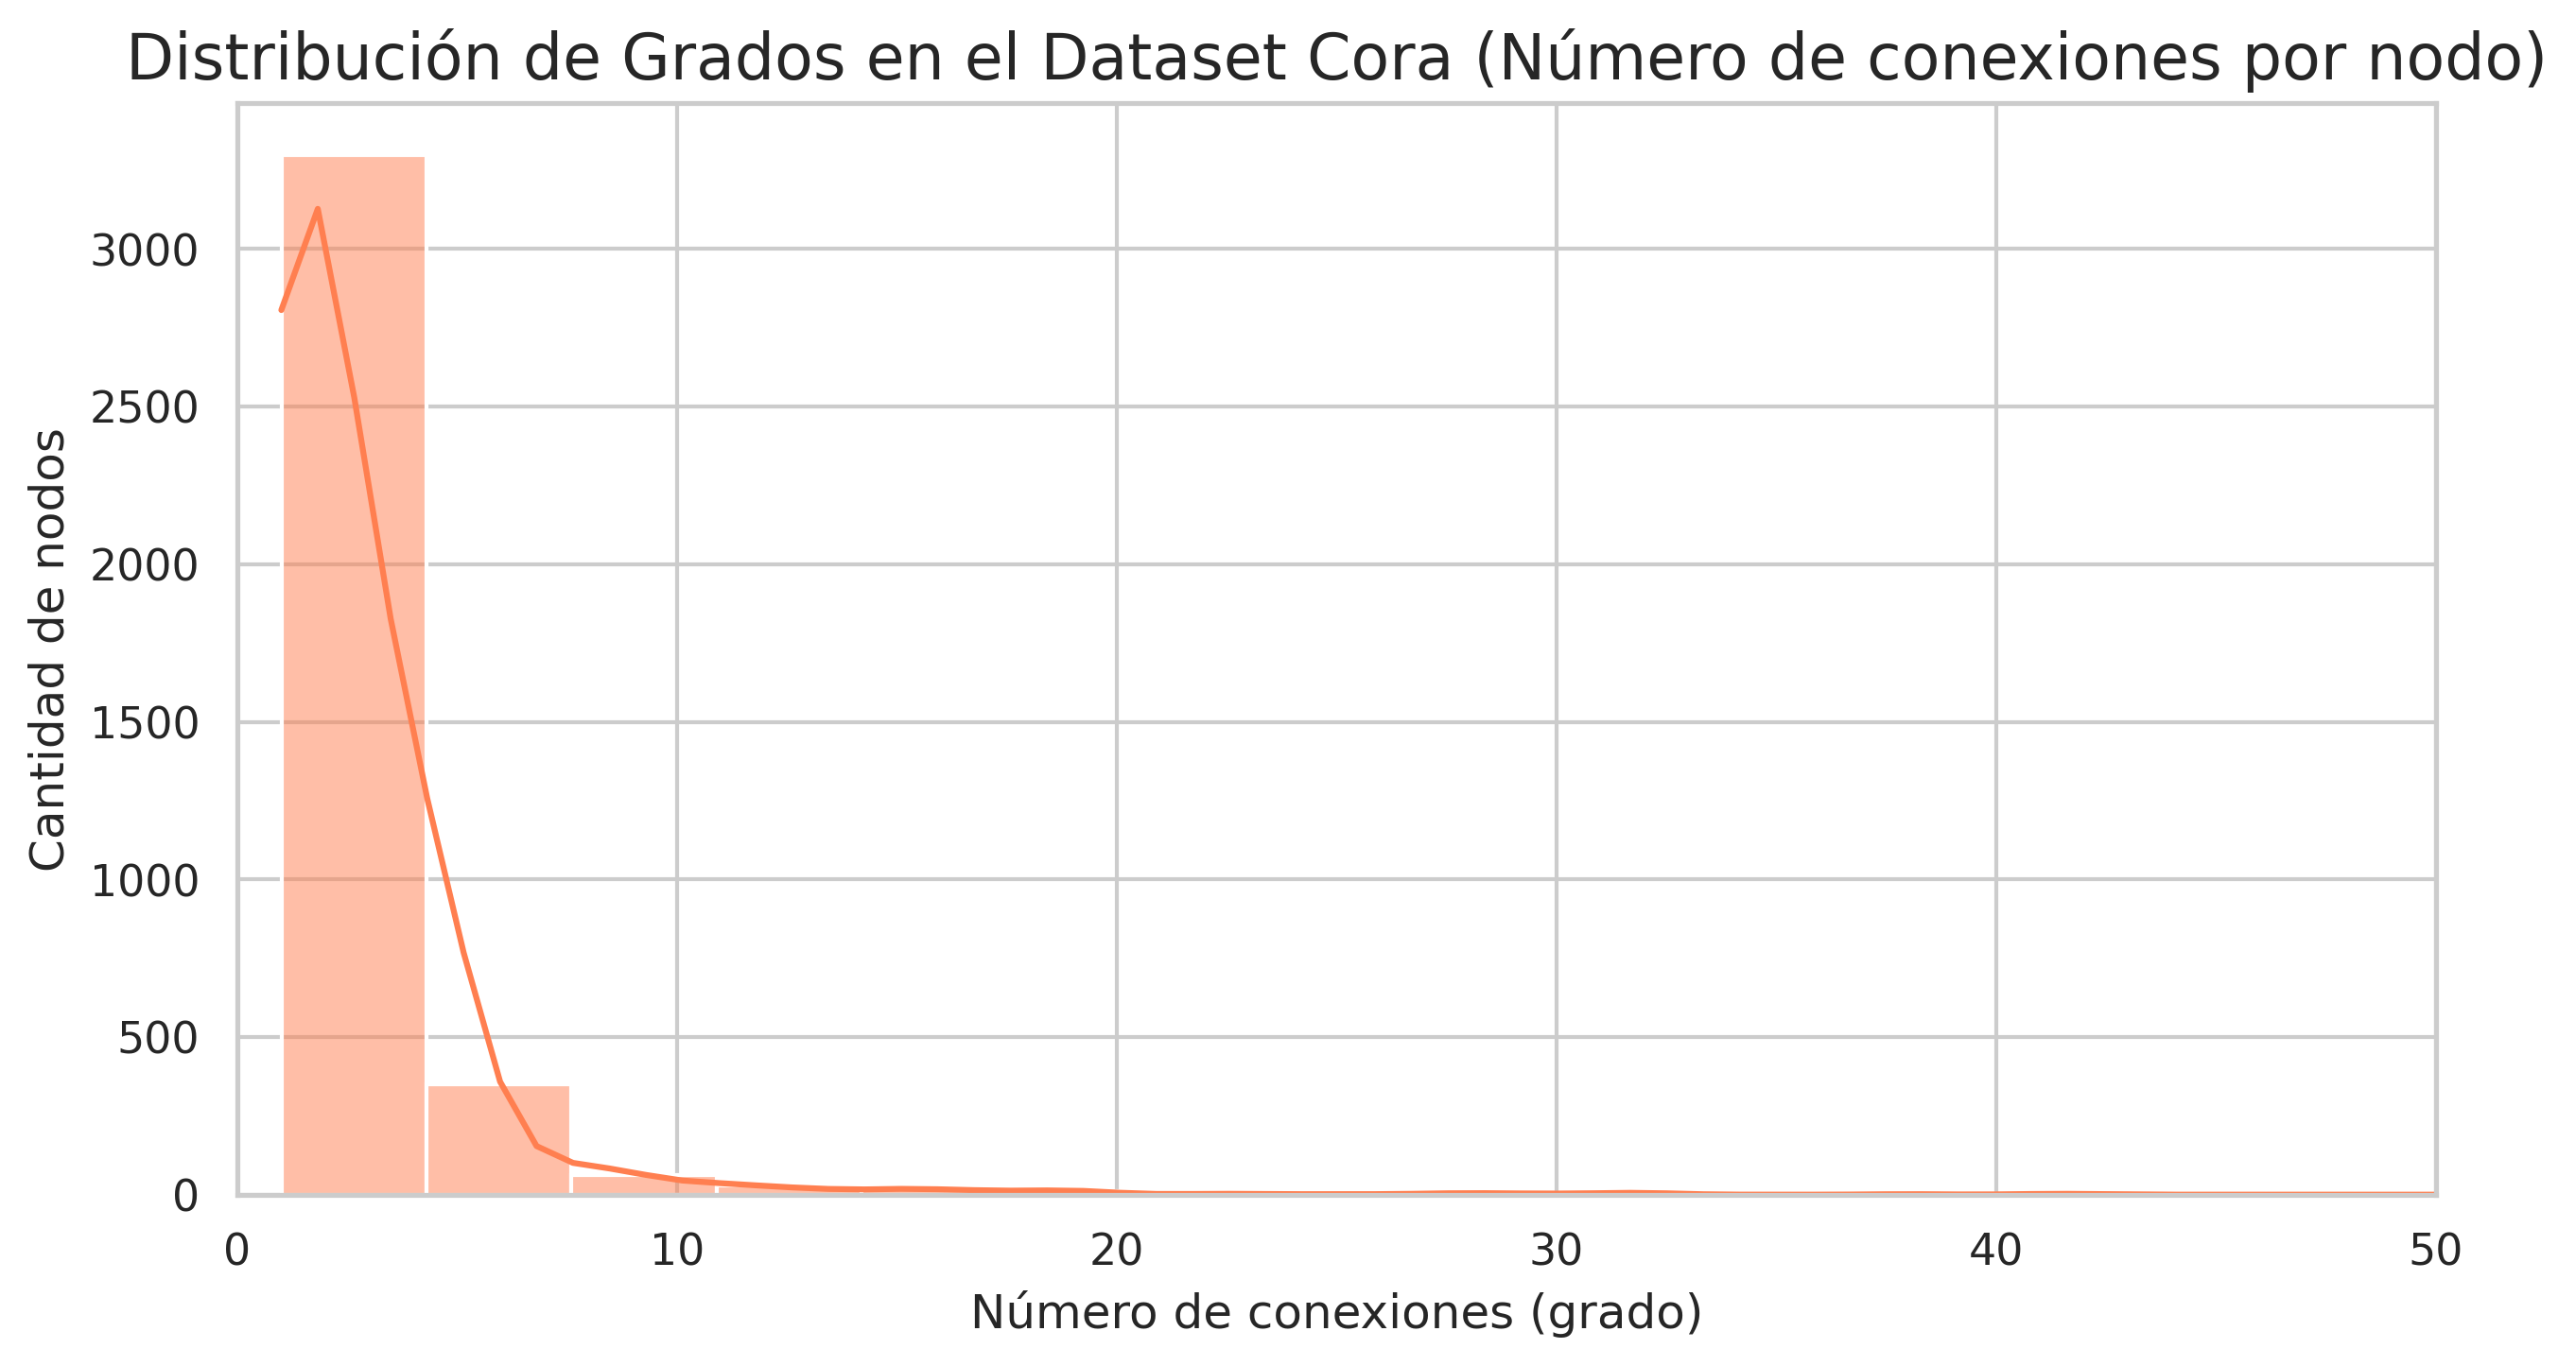
\includegraphics[width=\columnwidth]{figuras/distribucion_grados_cora.png}
  \caption{Distribución de grados del grafo de citación Cora}
  \label{fig:dist-grados}
\end{figure}

Para enriquecer la representación de cada publicación científica, se extrajeron tres métricas relacionales para cada nodo:

\begin{itemize}
    \item \textbf{Centralidad de Intermediación:} Elegida por su alta capacidad predictiva para identificar artículos que actúan 
    como ``puentes'' de información entre diversas áreas temáticas.
    
    \item \textbf{Coeficiente de Clustering:} Calculado para medir la tendencia de las publicaciones a agruparse en vecindarios densos
    interconectados.
    
    \item \textbf{Detección de Comunidades:} Se seleccionó el algoritmo de Louvain para agrupar latentemente el grafo, asignando a cada 
    artículo un identificador de la comunidad subyacente descubierta basándose exclusivamente en los enlaces.
\end{itemize}

La arquitectura final de los datos de entrada consolidó las 1433 variables del texto con las nuevas características relacionales en una 
única matriz.

\section*{C. Procedimiento de Entrenamiento}

Para asegurar una evaluación justa de la capacidad de generalización de los algoritmos de clasificación, el conjunto de datos se dividió
utilizando la validación por retención (\textit{holdout}), reservando el 80\% de los ejemplos para el entrenamiento de los modelos 
y el 20\% restante para las pruebas.

Como decisión de diseño, se aplicó un muestreo estratificado durante esta partición para preservar la proporción real de 
las clases y evitar sesgos derivados del desbalanceo del conjunto de datos.

El ajuste óptimo de los hiperparámetros de los cuatro modelos base se estructuró mediante una búsqueda en rejilla (\textit{GridSearchCV}). 
Durante este proceso, se aplicó una validación cruzada estratificada de 5 pliegues (5-fold cross validation) en el conjunto de 
entrenamiento para estimar el rendimiento a priori y seleccionar de forma robusta la mejor configuración de cada algoritmo.

\section{Resultados}

\subsection{Aprendizaje de Representaciones Latentes (Node2Vec)}

Para superar las limitaciones impuestas por la altísima dispersión del espacio de atributos nativos (98.73\% de ceros), se procedió a implementar un enfoque de aprendizaje de representaciones latentes
 en baja dimensión. Específicamente, se utilizó el algoritmo \textit{Node2Vec}, el cual emplea caminatas aleatorias (\textit{random walks}) para capturar la estructura topológica del grafo y la 
 homofilia de la red, generando un \textit{embedding} denso de solo 64 dimensiones para cada nodo.

Se aplicó la misma configuración experimental (validación cruzada de 5 pliegues y búsqueda en rejilla) sobre estas nuevas 64 variables continuas. Los resultados comparativos frente a la extracción manual
 de características se detallan en la Tabla \ref{tab:comparativa}.

\begin{table}[htbp]
\caption{Comparativa de F1-macro: Características Manuales vs. Node2Vec}
\begin{center}
\begin{tabular}{|l|c|c|}
\hline
\textbf{Modelo} & \textbf{Manual (1437 var.)} & \textbf{Node2Vec (64 var.)} \\
\hline
k-Vecinos (kNN) & 0.416 & \textbf{0.867} \\
Perceptrón (MLP) & 0.717 & 0.850 \\
Naive Bayes Gaussiano & 0.428 & 0.740 \\
Árbol de Decisión & \textbf{0.758} & 0.693 \\
\hline
\end{tabular}
\label{tab:comparativa}
\end{center}
\end{table}

\textit{Análisis Crítico:} El uso de \textit{embeddings} latentes provoca un cambio drástico en el rendimiento de los algoritmos. El modelo k-Vecinos más Cercanos (kNN), que presentaba el peor desempeño
 inicial, experimenta un resurgir extraordinario convirtiéndose en el mejor clasificador global (+0.109 de mejora en F1-macro). Este fenómeno se justifica teóricamente por la 
 "maldición de la dimensionalidad": mientras que en un espacio disperso de 1437 variables binarias las distancias matemáticas pierden su significado discriminativo, la distancia euclídea sobre 64 
 dimensiones densas refleja fielmente la verdadera proximidad estructural de los artículos en la red. Asimismo, modelos conexionistas como el MLP se benefician enormemente de las entradas continuas y 
 densas, alcanzando un 0.850.

En contraste, el Árbol de Decisión sufre un claro declive. Aunque este algoritmo sobresale trazando cortes ortogonales sobre variables binarias (presencia o ausencia de una palabra), resulta ineficiente
 para establecer fronteras de decisión jerárquicas óptimas en un espacio latente continuo, viéndose superado por modelos no lineales basados en distancias.

\begin{figure}[htbp]
\centerline{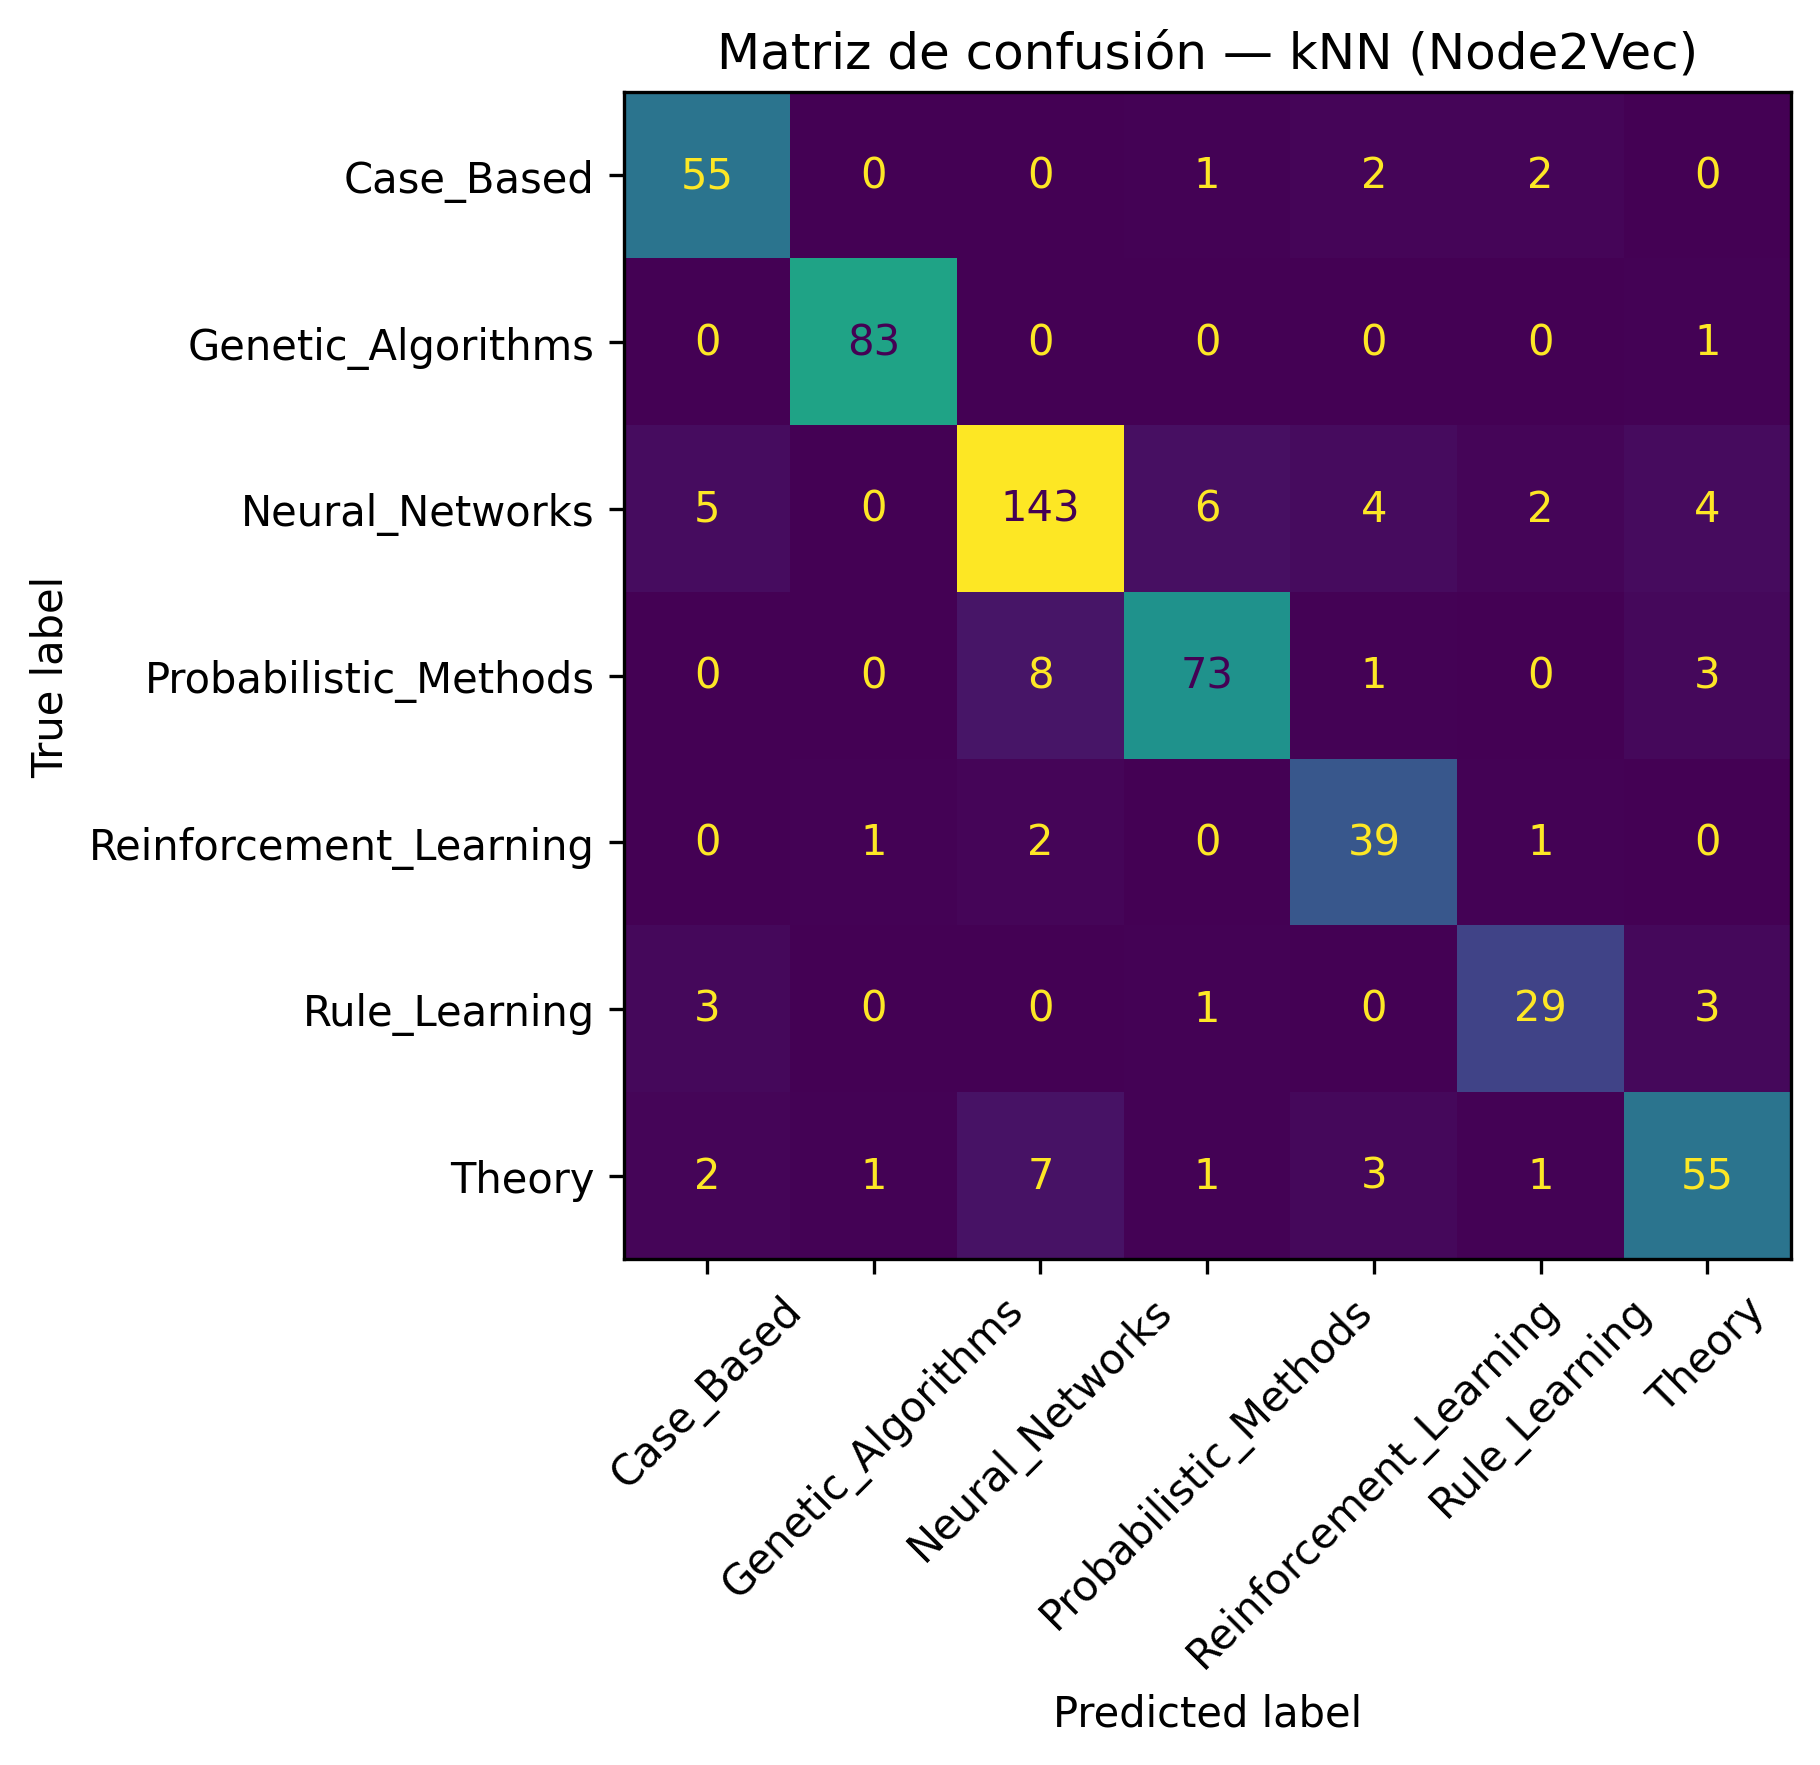
\includegraphics[width=\linewidth]{figuras/matriz_confusion_kNN_Node2Vec.png}}
\caption{Matriz de confusión obtenida para kNN utilizando embeddings de Node2Vec sobre el conjunto de prueba.}
\label{fig:matriz_knn}
\end{figure}

\textit{Análisis de Sobreajuste (Overfitting):} Para confirmar la capacidad de generalización del modelo base seleccionado y descartar problemas de sobreajuste, se analizó la brecha de rendimiento entre
 la fase de validación cruzada y la fase de prueba. El Árbol de Decisión obtuvo un \textit{F1-macro} medio de 0.7477 durante la validación cruzada estratificada de 5 pliegues, frente al 0.7588 obtenido 
 en el conjunto de prueba aislado. Esta mínima desviación confirma que la configuración de hiperparámetros elegida (criterio Gini, profundidad máxima de 20 y división mínima de 5 muestras) logra abstraer 
 los patrones del dataset Cora sin memorizar el ruido de entrenamiento.


\section{Conclusiones}

El trabajo desarrollado permite concluir que la estructura matemática de los enlaces en redes de citación científica aporta una información predictiva fundamental que los modelos tradicionales ignoran.
 Aunque la extracción manual de métricas estructurales (centralidad y comunidades) combinada con particionado jerárquico (Árboles de Decisión) establece una línea base sólida (F1-macro de 0.758), 
 el aprendizaje de representaciones latentes demuestra ser inmensamente superior.

Tras la optimización, \textbf{el modelo definitivo seleccionado es el clasificador k-Vecinos más Cercanos (kNN) alimentado con representaciones latentes generadas por Node2Vec}. Este enfoque logra
 comprimir el espacio de características de 1437 variables a solo 64 dimensiones densas, mitigando la dispersión del texto y alcanzando un F1-macro sobresaliente de 0.867 en el conjunto de prueba, 
 lo que supone una mejora de casi 11 puntos porcentuales respecto a la línea base.

\textbf{Trabajo Futuro:}
Para culminar el análisis relacional, los esfuerzos del próximo sprint se centrarán exclusivamente en la técnica de validación de atributos:
\begin{itemize}
    \item \textbf{Análisis de Correlaciones y Selección de Características:} Se aplicarán pruebas estadísticas sobre la matriz de 1437 características manuales originales. El objetivo será filtrar el 
    ruido eliminando palabras poco informativas y evaluar si un modelo base altamente depurado es capaz de acercarse al rendimiento excepcional obtenido por el aprendizaje latente de Node2Vec.
\end{itemize}

\begin{thebibliography}{00}
\bibitem{b1} P. Sen, G. Namata, M. Bilgic, L. Getoor, B. Gallagher, and T. Eliassi-Rad, "Collective Classification in Network Data," \textit{AI Magazine}, vol. 29, no. 3, pp. 93-106, 2008.
\bibitem{b2} S. Fortunato, "Community detection in graphs," \textit{Physics Reports}, vol. 486, no. 3-5, pp. 75-174, 2010.

\end{thebibliography}


\end{document}
